\documentclass{article}
\usepackage[utf8]{inputenc}
\usepackage[margin=0.8in]{geometry}
\usepackage{graphicx}
\usepackage{wrapfig}

\title{Practica 1 + 2 - BASES DE DATOS 2}
\author{
  Hayk Kocharyan\\
  757715@unizar.es
  \and
  Pedro Tamargo Allué\\
  758267@unizar.es
  \and
  Jesús Villacampa Sagaste\\
  755739@unizar.es
  \and
  Juan José Tambo Tambo\\
  755742@unizar.es
}

\date{\today}

\usepackage{natbib}
\usepackage{graphicx}
% Para los codigos
\usepackage{listings}

\begin{document}

\maketitle

%\input{insbox}
\tableofcontents

\newpage 

\section{Esfuerzos invertidos}
Los esfuerzos invertidos por cada integrante del equipo son:
\begin{itemize}
\item Hayk:
\item Juan José:
\item Jesús:
\item Pedro: 
\end{itemize}

\section{Configuración de la máquina virtual}
Para la realización de esta práctica se han utilizado las máquinas de 32 y 64 bits y su configuración ha sido igual para ambas.\\

Para la instalación de los \emph{SGBD} se debía conectar por medio de ssh  desde la máquina local utilizando $ssh -Xroot@dirmaquina$ para poder utilizar herramientas gráficas necesarias. Para ello, se debe configurar las interfaces de red de las máquinas de la siguiente manera:\\
Desde VirtualBox, añadir un adaptador “Host-only Adapter”:\\
Configuración->Network->Adapter2->Host-only Adapter (Name: vboxnet0).
\\
Para que aparezca vboxnet0:\\
file->Host Network Adapter->create
\\
Una vez realizado lo anterior, desde la máquina virtual, se debe configurar el archivo /etc/network/interfaces y modificar la interfaz eth1 de la siguiente manera:\\
\begin{figure}[h!]
	\centering
		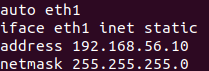
\includegraphics[scale=1.5]{images/interfacesred.png}
			\caption{Depliegue del sistema}
\end{figure}


\section{Instalación y administración básica de los SGBD}

\section{Comentarios acerca de las licencias}

\section{Diseño conceptual de la base de datos}

\section{Diseño lógico de una base de datos relacional}
\subsection{Implementación con el modelo relacional}

Para la transformación del del Diagrama Entidad-Relación en un modelo relacional se ha convertido la generalización de Cuenta en dos tablas, sus subtablas $Cuenta\_ahorro$ y $Cuenta\_corriente$, y la generalización de Transacción en sus dos subtablas Transferencia y Operación.\\

Las relaciones entre las entidades se han traducido en función de su cardinalidad. Las relaciones \emph{(M:N)} se han traducido en una nueva relación.\\

\textbf{Para la implementación en el SGBD Oracle se han utilizado tablas las tablas especificadas anteriormente y se han establecido las restricciones de integridad referencial a las tablas que hacen referencia a otras. ??}

\section{Implementación con el modelo relacional}
\subsection{Implementación con el modelo objeto/relacional}
\subsubsection{Oracle}
Para la implementación del modelo \emph{OR} con \emph{Oracle} se han creado tantos tipos como entidades teníamos en el Diagrama Entidad-Relación, además para reflejar las relaciones bidireccionales entre dos entidades se han creado otros tipos (listaCuentas, listaPropietarios y realizadasUdt) como tablas de referencias a otros tipos ya creados anteriormente.
\\
Tras la creación de los tipos, procedemos a crear las tablas de los mismos. Oracle tiene como particularidad que no existen jerarquías de tablas, es decir, crearemos una tabla para el supertipo de la jerarquía y realizaremos las restricciones de integridad referencial mediante las cláusulas \emph{FOREIGN KEY} en las tablas y \emph{SCOPE} en las tablas anidadas.
\\

\subsubsection{PostgreSQL}
Cosas de PostgreSQL
\\

\subsubsection{DB2}
Cosas de DB2
\\

\section{Diseño lógico de una base de datos objeto/relacional}

\section{Implementación con el modelo objeto/relacional}

\section{Generación de datos y pruebas}

\section{Implementación con db4o}

\section{Comparación de los SGBD}


\end{document}
